\documentclass[aspectratio=169]{beamer}
\usetheme{Madrid}
\usecolortheme{default}
\usepackage[utf8]{inputenc}
\usepackage[portuguese]{babel}
\usepackage{tabularx}
\usepackage{booktabs}
\usepackage[most]{tcolorbox}
\usepackage{graphicx}
\graphicspath{{.}{../Figuras/}}

\title[Virtualização, Nuvem e Contêineres]{Virtualização, Nuvem e Contêineres}
\subtitle[]{Arquitetura, modelos de serviço, segurança e eficiência energética}
\author[Marco, Murilo e Rodrigo]{Marco Antônio Cottorello Henry \and Murilo de Souza Neves \and Rodrigo Macedo da Silva Junior}
\date{Outubro 2026}

% divisor de secao
\newcommand{\divisor}[1]{%
\begin{frame}
  \begin{center}
    \begin{tcolorbox}[
        width=0.97\textwidth,
        colback=structure.fg!90!black,
        colframe=structure.fg!80!black,
        coltext=white,
        boxrule=0pt,
        arc=3mm,
        drop shadow,
        halign=center,
        top=4mm,
        bottom=4mm
      ]
      {\Large #1\par}
    \end{tcolorbox}
  \end{center}
\end{frame}}

\begin{document}

\begin{frame}
    \titlepage
\end{frame}

\begin{frame}{O que a apresentação cobre}
  \begin{enumerate}
    \setcounter{enumi}{0}
    \item \textbf{Computação em nuvem}. O que define uma nuvem e o que separa IaaS, PaaS e SaaS.
    \item \textbf{OpenStack}. Como se constrói uma nuvem de infraestrutura própria.
    \setcounter{enumi}{3}
    \item \textbf{Docker}. Como o contêiner é isolado e como ele se conecta em rede.
    \setcounter{enumi}{5}
    \item \textbf{Segurança} em cloud e contêineres.
    \item \textbf{Eficiência energética} em data centers.
  \end{enumerate}
  \vspace{0.3cm}
  \begin{tcolorbox}[colback=structure.fg!10, colframe=structure.fg!60, arc=2mm]
    Os temas formam uma pilha. A nuvem define o modelo de serviço, o OpenStack implementa a oferta de infraestrutura, o Docker empacota as cargas, e as duas últimas partes analisam as consequências dessa escolha.
  \end{tcolorbox}
\end{frame}

% =====================================================================
\divisor{1. Computação em Nuvem}

\begin{frame}{A definição do NIST}
  \begin{tcolorbox}[colback=structure.fg!10, colframe=structure.fg!60, arc=2mm]
    Modelo que habilita acesso ubíquo, conveniente e sob demanda, via rede, a um conjunto compartilhado de recursos computacionais configuráveis, rapidamente provisionados e liberados com esforço mínimo de gerenciamento ou de interação com o provedor.
    \hfill {\footnotesize NIST SP 800-145}
  \end{tcolorbox}
  \vspace{0.3cm}
  \textbf{Cinco características essenciais, todas obrigatórias}
  \begin{columns}[T]
    \begin{column}{0.48\textwidth}
      \begin{itemize}
        \item Autoatendimento sob demanda
        \item Amplo acesso à rede
        \item Agrupamento de recursos
      \end{itemize}
    \end{column}
    \begin{column}{0.48\textwidth}
      \begin{itemize}
        \item Elasticidade rápida
        \item Serviço medido
      \end{itemize}
    \end{column}
  \end{columns}
  \vspace{0.2cm}
  {\footnotesize Falta uma delas e o sistema não é nuvem pela definição. Hospedagem com capacidade fixa e sem medição é hospedagem.}
\end{frame}

\begin{frame}{Modelos de serviço e a fronteira de controle}
  \begin{figure}
    \centering
    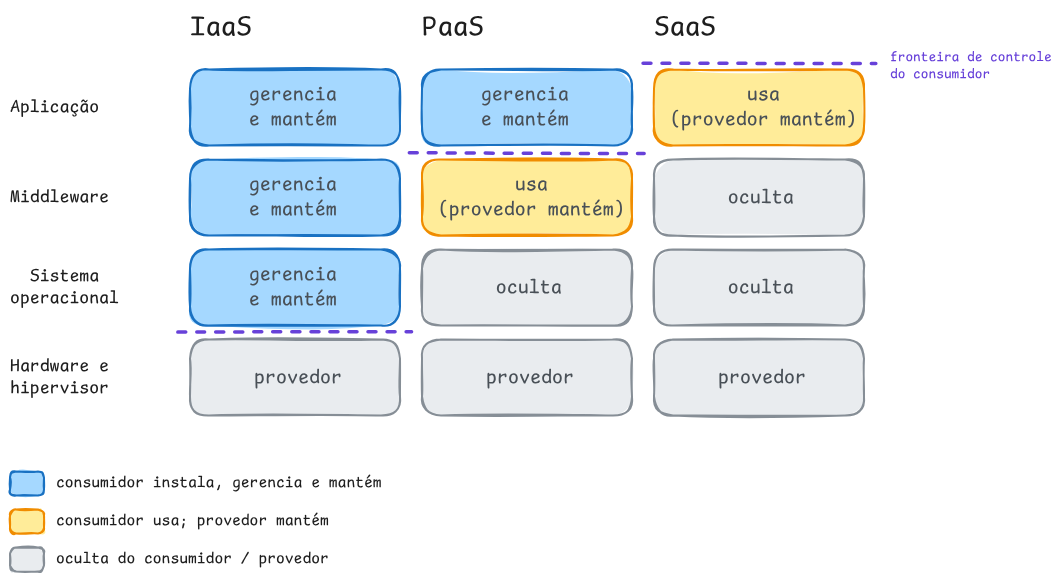
\includegraphics[height=0.68\textheight]{modelosdeservico.png}
  \end{figure}
  \vspace{-0.3cm}
  {\footnotesize A fronteira de controle sobre a pilha é o que separa os três modelos, e não a quantidade de infraestrutura pronta. \hfill NIST SP 500-292, Fig. 8}
\end{frame}

\begin{frame}{Modelos de implantação}
  O critério é o \textbf{grau de exclusividade} do recurso, e não a localização física.
  \vspace{0.25cm}
  \begin{columns}[T]
    \begin{column}{0.48\textwidth}
      \textbf{Pública}
      \begin{itemize}
        \item Uso aberto ao público
        \item Existe nas instalações do provedor
      \end{itemize}
      \textbf{Privada}
      \begin{itemize}
        \item Uso exclusivo de uma organização
        \item Pode ser operada por terceiro e ficar fora das instalações
      \end{itemize}
    \end{column}
    \begin{column}{0.48\textwidth}
      \textbf{Comunitária}
      \begin{itemize}
        \item Uso exclusivo de organizações com preocupações comuns
      \end{itemize}
      \textbf{Híbrida}
      \begin{itemize}
        \item Composição de duas ou mais, que permanecem distintas
        \item Ligadas por tecnologia de portabilidade, como \textit{cloud bursting}
      \end{itemize}
    \end{column}
  \end{columns}
  \vspace{0.15cm}
  {\footnotesize Privada não significa dentro de casa. Híbrida não é usar um pouco de cada, exige portabilidade entre as nuvens.}
\end{frame}

\begin{frame}{Onde entram OpenStack e Docker}
  \begin{figure}
    \centering
    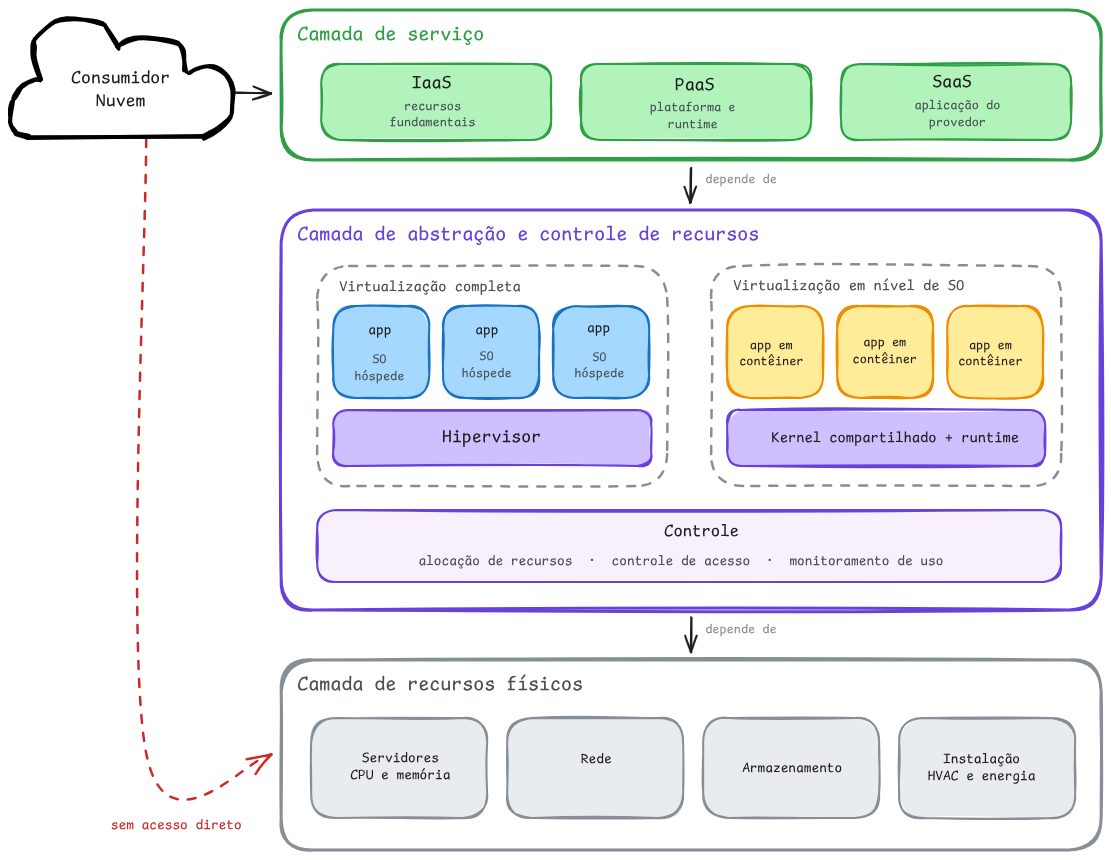
\includegraphics[height=0.74\textheight]{camadasabstracao.png}
  \end{figure}
  \vspace{-0.15cm}
  {\footnotesize Os dois próximos temas moram na camada do meio. O consumidor acessa a camada de serviço e nunca os recursos físicos.}
\end{frame}

% =====================================================================
\divisor{2. OpenStack}

\begin{frame}{O problema e a solução}
  \begin{columns}[T]
    \begin{column}{0.48\textwidth}
      \textbf{Cinquenta servidores sem plataforma}
      \begin{itemize}
        \item Pedido abre uma solicitação
        \item Um administrador escolhe o servidor, instala o sistema e configura a rede
        \item Horas ou dias, com dependência de pessoas
        \item Consumo não medido
      \end{itemize}
    \end{column}
    \begin{column}{0.48\textwidth}
      \textbf{Os mesmos servidores com OpenStack}
      \begin{itemize}
        \item Pedido vira requisição de API
        \item A plataforma escolhe o nó, cria a instância a partir de uma imagem e conecta a rede
        \item Segundos, sem intermediação
        \item Consumo atribuído ao projeto
      \end{itemize}
    \end{column}
  \end{columns}
  \vspace{0.3cm}
  \begin{tcolorbox}[colback=structure.fg!10, colframe=structure.fg!60, arc=2mm]
    Conjunto de programas de código aberto que transforma servidores comuns em uma nuvem de infraestrutura. É o que a AWS oferece como serviço, construído no data center próprio.
  \end{tcolorbox}
\end{frame}

\begin{frame}{Arquitetura modular}
  Todo serviço da plataforma repete o mesmo formato interno.
  \vspace{0.2cm}
  \begin{columns}[T]
    \begin{column}{0.52\textwidth}
      \begin{itemize}
        \item \textbf{Processo de API}, porta de entrada que escuta requisições
        \item \textbf{Processos de trabalho}, que executam a tarefa, muitas vezes em outras máquinas
        \item \textbf{Banco de dados} próprio, que guarda o estado
        \item \textbf{Fila AMQP}, que entrega tarefas aos processos de trabalho
      \end{itemize}
    \end{column}
    \begin{column}{0.44\textwidth}
      \begin{tcolorbox}[colback=structure.fg!10, colframe=structure.fg!60, arc=2mm, fontupper=\footnotesize]
        \textbf{Dois níveis de comunicação}
        \vspace{0.15cm}

        Dentro de um serviço, fila AMQP.

        Entre serviços distintos, chamadas de API pública.
        \vspace{0.1cm}

        Todos autenticam no mesmo serviço de identidade.
      \end{tcolorbox}
    \end{column}
  \end{columns}
  \vspace{0.2cm}
  {\footnotesize Consequência prática. Cada serviço é atualizado ou escalado de forma independente, desde que a API continue a mesma.}
\end{frame}

\begin{frame}{Os serviços e a criação de uma instância}
  \footnotesize
  \begin{tabularx}{\textwidth}{@{} l X @{}}
    \toprule
    \textbf{Serviço} & \textbf{Responde por} \\
    \midrule
    Keystone  & Identidade, autenticação e permissões por projeto \\
    Glance    & Catálogo de imagens, o sistema de arquivos inicial da instância \\
    Nova      & Criação e ciclo de vida das instâncias \\
    Neutron   & Redes, sub-redes, roteadores, endereços e grupos de segurança \\
    Placement & Inventário de recursos livres de cada nó \\
    \bottomrule
  \end{tabularx}
  \vspace{0.3cm}
  \normalsize
  \textbf{Sequência de uma criação}
  \begin{enumerate}
    \item Keystone confirma identidade e papel no projeto
    \item Placement indica o nó com recursos livres
    \item Glance entrega a imagem de origem
    \item Neutron provisiona a rede da interface
    \item O hipervisor do nó escolhido executa a máquina virtual
  \end{enumerate}
  {\footnotesize O OpenStack coordena e delega. A execução continua sendo do hipervisor.}
\end{frame}

% =====================================================================
\divisor{4. Docker}

\begin{frame}{A engine não é um processo único}
  \begin{columns}[T]
    \begin{column}{0.54\textwidth}
      \begin{itemize}
        \item \texttt{docker}, cliente que traduz comandos em requisições REST
        \item \texttt{dockerd}, daemon que gerencia imagens, contêineres, redes e volumes
        \item \texttt{containerd}, ciclo de vida e armazenamento em camadas
        \item \texttt{containerd-shim}, processo pai de cada contêiner
        \item \texttt{runc}, cria o processo isolado e sai de cena
      \end{itemize}
    \end{column}
    \begin{column}{0.42\textwidth}
      \begin{tcolorbox}[colback=black!88, coltext=white, colframe=black, arc=2mm, fontupper=\tiny\ttfamily]
        \$ ps -eo pid,ppid,comm \\[2pt]
        \ \ 1019 \ \ \ \ \ 1 containerd \\
        \ \ 1147 \ \ \ \ \ 1 dockerd \\
        \ 39649 \ \ \ \ \ 1 containerd-shim \\
        \ 39673 \ 39649 nginx
      \end{tcolorbox}
      {\scriptsize O \textit{shim} tem PPID 1, não 1147. Por isso o daemon reinicia sem derrubar contêineres.}
    \end{column}
  \end{columns}
  \vspace{0.2cm}
  {\footnotesize Especificações da OCI separam o formato da imagem da forma de executá-la, o que dá interoperabilidade entre \textit{runtimes}.}
\end{frame}

\begin{frame}{Isolamento. Namespaces e cgroups}
  \begin{columns}[T]
    \begin{column}{0.5\textwidth}
      \textbf{Namespaces, o que o processo vê}
      \begin{itemize}
        \item \textbf{pid}, processo inicial recebe o identificador 1
        \item \textbf{mnt}, árvore de montagem própria
        \item \textbf{net}, pilha de rede própria
        \item \textbf{ipc}, \textbf{uts}, \textbf{user}, \textbf{cgroup}, \textbf{time}
      \end{itemize}
    \end{column}
    \begin{column}{0.46\textwidth}
      \textbf{Cgroups, quanto ele consome}
      \begin{itemize}
        \item Processador, memória, disco e número de processos
      \end{itemize}
      \begin{tcolorbox}[colback=black!88, coltext=white, colframe=black, arc=2mm, fontupper=\tiny\ttfamily]
        \$ docker run --memory 64m --cpus 0.5 \\
        \ \ alpine cat /sys/fs/cgroup/memory.max \\[2pt]
        67108864 \\
        \$ cat /sys/fs/cgroup/cpu.max \\[2pt]
        50000 100000
      \end{tcolorbox}
    \end{column}
  \end{columns}
  \vspace{0.25cm}
  \begin{tcolorbox}[colback=red!8, colframe=red!55, arc=2mm, fontupper=\footnotesize]
    O kernel permanece compartilhado e a interface de chamadas de sistema continua comum a todos os contêineres. Namespaces e cgroups são mecanismo de isolamento, não fronteira de segurança equivalente à de uma máquina virtual.
  \end{tcolorbox}
\end{frame}

\begin{frame}{Redes locais do Docker}
  Todo modelo deriva do tratamento dado ao \textit{namespace} de rede.
  \vspace{0.15cm}
  \footnotesize
  \begin{tabularx}{\textwidth}{@{} l X X @{}}
    \toprule
    \textbf{Modelo} & \textbf{Namespace de rede} & \textbf{Exposição} \\
    \midrule
    \textit{bridge} padrão & próprio, ligado à ponte \texttt{docker0} & mascaramento na saída, publicação de porta na entrada \\
    \textit{bridge} do usuário & próprio, ponte dedicada, DNS interno & igual à padrão, com resolução por nome \\
    \textit{host} & compartilhado com o hospedeiro & direta, na porta real do hospedeiro \\
    \textit{none} & próprio e vazio & nenhuma \\
    \textit{macvlan} e \textit{ipvlan} & exposto à rede física & dispositivo na rede local \\
    \bottomrule
  \end{tabularx}
  \vspace{0.25cm}
  \normalsize
  \begin{columns}[T]
    \begin{column}{0.52\textwidth}
      {\footnotesize A assimetria da \textit{bridge}. O contêiner alcança a Internet sem configuração, mas só é alcançável de fora com publicação de porta.
      \vspace{0.15cm}

      O kernel compartilhado é o que torna o contêiner denso, e é o que amplia a superfície de ataque. É o ponto de partida das duas partes seguintes.}
    \end{column}
    \begin{column}{0.44\textwidth}
      \begin{tcolorbox}[colback=black!88, coltext=white, colframe=black, arc=2mm, fontupper=\tiny\ttfamily]
        \# bridge padrão \\
        nameserver 172.17.0.1 \\
        getent hosts web \ \ (vazio) \\[3pt]
        \# bridge do usuário \\
        nameserver 127.0.0.11 \\
        getent hosts web \ \ 172.21.0.2
      \end{tcolorbox}
    \end{column}
  \end{columns}
\end{frame}


\begin{frame}
    \begin{center}
        \begin{tcolorbox}[
                width=0.97\textwidth,
                colback=structure.fg!90!black, 
                colframe=structure.fg!80!black, 
                coltext=white,
                boxrule=0pt,
                arc=3mm,
                drop shadow,
                halign=center,
                top=4mm,
                bottom=4mm
            ]
            {\Large 6. Segurança no Ambiente de Cloud e Contêineres\par}

        \end{tcolorbox}
    \end{center}
\end{frame}

\begin{frame}{A Transição da Virtualização}
    \textbf{De Máquinas Virtuais para Contêineres:}
    \vspace{0.2cm}
    \begin{columns}[T]
        \begin{column}{0.48\textwidth}
            \textbf{Máquinas Virtuais}
            \begin{itemize}
                \item Sistema convidado completo.
                \item Alto \textit{overhead} de hardware.
                \item Isolamento robusto via hipervisor.
            \end{itemize}
        \end{column}
        \begin{column}{0.48\textwidth}
            \textbf{Contêineres}
            \begin{itemize}
                \item Compartilham o kernel hospedeiro.
                \item Alta densidade de consolidação.
                \item Risco elevado de ataques de escape em ambientes \textit{multitenant}.
            \end{itemize}
        \end{column}
    \end{columns}
\end{frame}

\begin{frame}{De Máquinas Virtuais para Contêineres:}
    \begin{figure}
        \centering
        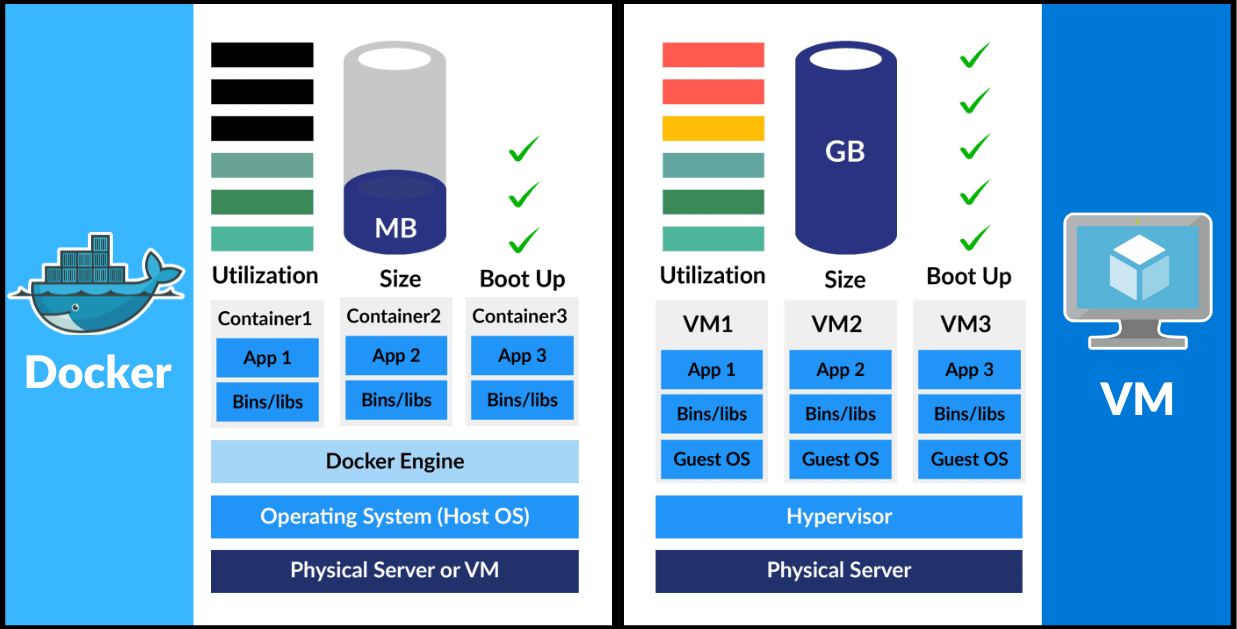
\includegraphics[width=0.8\linewidth]{vmxcont.png}
        \label{fig:placeholder}
    \end{figure} 
\end{frame}

\begin{frame}{Problemas do uso de contêineres}
    \begin{itemize}
        \item Kerner Compartilhado: Ausência de hipervisor dedicado. Interação direta com o SO hospedeiro.
        \item Cadeia de Ferramentas: Múltiplos vetores de ataque. Desde a construção da imagem até a execução.
    \end{itemize}

    \begin{columns}[T]
        \begin{column}{0.48\textwidth}
            \textbf{Máquinas Virtuais}
            \begin{itemize}
                \item Kernel dedicado isolado.
                \item Barreira física do Hipervisor.
                \item Menor superfície de ataque.
            \end{itemize}
        \end{column}
        \begin{column}{0.48\textwidth}
            \textbf{Contêineres}
            \begin{itemize}
                \item Compartilhamento do kernel hospedeiro.
                \item Isolamento apenas lógico (nível SO).
                \item Maior exposição em caso de fuga (breakout).
            \end{itemize}
        \end{column}
    \end{columns}
\end{frame}

\begin{frame}{Primitivas de Contenção do Kernel}
    Como controlar privilégios e evitar vazamentos?
    \vspace{0.5cm}
    \begin{itemize}
        \item \textbf{Namespaces:} Isolam a visibilidade de recursos globais (PIDs, redes e montagens).
        \item \textbf{Cgroups:} Contabilizam e limitam o consumo físico (CPU, RAM).
        \item \textbf{Rootless Containers:} Execução sem privilégios de superusuário.
        \item \textbf{Seccomp:} Restrição estrita de chamadas de sistema (\textit{syscalls}).
    \end{itemize}
\end{frame}

\begin{frame}{Cadeia de Suprimentos e Zero Trust}
    Vulnerabilidades de Imagens e Tráfego \textit{Leste-Oeste}
    \vspace{0.5cm}
    \begin{itemize}
        \item \textbf{Imagens Distroless:} Artefatos enxutos sem \textit{shell} (mitiga instrumentação invasora).
        \item \textbf{Microssegmentação:} Políticas de rede configuradas como \textit{default-deny}.
        \item \textbf{eBPF:} Inspeção de pacotes de alta performance no espaço de kernel.
        \vspace{0.3cm}
        \item \textit{Exemplo prático:} A campanha GhostAction (2026) extraiu segredos devido à ausência dessas contenções de rede em esteiras CI/CD efêmeras.
    \end{itemize}
\end{frame}

\begin{frame}{Campanha GhostAction}
    \begin{figure}
        \centering
        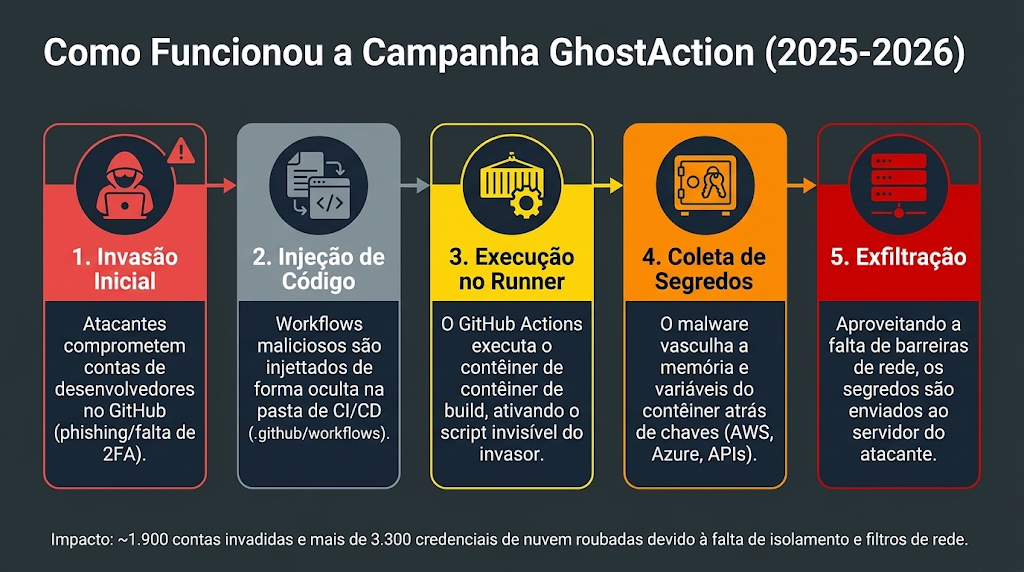
\includegraphics[width=0.8\linewidth]{ghostaction.png}
        \label{fig:placeholder}
    \end{figure}
\end{frame}

\begin{frame}
    \begin{center}
        \begin{tcolorbox}[
                width=0.97\textwidth,
                colback=structure.fg!90!black, 
                colframe=structure.fg!80!black, 
                coltext=white,
                boxrule=0pt,
                arc=3mm,
                drop shadow,
                halign=center,
                top=4mm,
                bottom=4mm
            ]
            {\Large 7. Eficiência Energética em Data Centers\par}

        \end{tcolorbox}
    \end{center}
\end{frame}

\begin{frame}{O Desafio do Desperdício Energético}
    O indicador \textbf{PUE} (Power Usage Effectiveness):
    \begin{equation*}
        PUE = \frac{P_{\text{Total da Instalação}}}{P_{\text{Equipamentos de TI}}}
    \end{equation*}
    
    \vspace{0.5cm}
    \textbf{A limitação do PUE:}
    \begin{itemize}
        \item Não mede a eficiência interna do servidor.
        \item \textbf{O Paradoxo da Ociosidade:} Servidores com 10\%-20\% de uso de CPU ainda consomem até 60\% de sua potência máxima.
    \end{itemize}
\end{frame}

\begin{frame}{Consolidação e Gestão Térmica}
    Para combater a potência ociosa, e melhorar gestão térmica (ASHRAE TC 9.9), concentramos cargas:
    \vspace{0.5cm}
    \begin{enumerate}
        \item \textbf{Bin Packing:} Consolidação dinâmica via contêineres para desligar nós excedentes.
        \item \textbf{Contenção de Corredores:} Isolamento aerodinâmico quente/frio.
        \item \textbf{Liquid Cooling:} Resfriamento líquido direto no componente ou por imersão
    \end{enumerate}
    
\end{frame}

\begin{frame}{Síntese Integradora: Segurança $\times$ Energia}
    \small
    \renewcommand{\arraystretch}{1.3}
    \begin{tabularx}{\textwidth}{@{}l X X@{}}
        \toprule
        \textbf{Dimensão} & \textbf{Solução Técnica} & \textbf{Impacto Cruzado} \\
        \midrule
        Kernel & \textit{Namespaces, cgroups, Rootless} & Consolidação alta sem gasto de VMs. \\
        Rede & Imagens \textit{Distroless}, \textit{eBPF} & Menos uso de CPU/Rede. \\
        Alocação & Consolidação (\textit{Bin Packing}) & Reduz $P_{\text{TI}}$, exige contenção lógica forte. \\
        Térmica & \textit{Liquid Cooling}, Contenção & Reduz refrigeração sob consolidação. \\
        \bottomrule
    \end{tabularx}
\end{frame}

\begin{frame}{O Cenário Global e Brasileiro}
    A urgência impulsionada por IA e Hiperescala:
    \vspace{0.5cm}
    \begin{itemize}
        \item \textbf{945 TWh:} Projeção global de consumo do setor até 2030 (IEA).
        \item \textbf{5 GW: } Projeção média de ONS de carga exclusiva de data centers no Sistema Interligado Nacional (SIN) até 2030 (ONS)
        \item \textbf{+40 kW/rack:} Densidade térmica atual de novos complexos, tornando o resfriamento tradicional a ar obsoleto.
    \end{itemize}
    \vspace{0.5cm}
    \centering
\end{frame}

\begin{frame}
    \begin{center}
        \begin{tcolorbox}[
                width=0.97\textwidth,
                colback=structure.fg!90!black, 
                colframe=structure.fg!80!black, 
                coltext=white,
                boxrule=0pt,
                arc=3mm,
                drop shadow,
                halign=center,
                top=4mm,
                bottom=4mm
            ]
            {\Large Obrigado!\par}

        \end{tcolorbox}
    \end{center}
\end{frame}

\end{document}